\subsection{Chargenrückverfolgung} \label{sec:batch-traceability}
\textcolor{red}{Notwendigkeit einer Charge erläutern auf Grund der Gruppierung von vielen Einzelprodukten eben zu einer Charge.}

\subsubsection{Definition Charge}

Eine \textit{Charge} bezeichnet eine Ansammlung eines Produkts, welche unter gleichen Bedingungen produziert wurde. Bei dem Produkt kann es sich beispielsweise um Werkstoffe, Bauteile, Baugruppen oder Endprodukte handeln. Die Begriffe \textit{Los} oder \textit{Partie} werden oft als Synonym für \textit{Charge} verwendet. Einige Branchen sind bei der Produktion auf die Erzeugung definierter \textit{Chargen} zugeschnitten. Diese Chargenproduktion, die auch diskontinuierliche Produktion genannt wird, zeichnet sich durch einen zeitlich unterbrochenen Materialfluss aus. So kann ein Produktionsgefäß mit unterschiedlichen Rohstoffen befüllt und anschließend verarbeitet werden. In der diskontinuierlichen Produktion versteht man daher unter einer \textit{Charge} eine Menge eines Erzeugnisses, welche in einem Produktionsgang gefertigt worden ist und identische Kennzeichen in Bezug auf Materialzusammensetzung, Fertigungsprozess und Produktqualität aufweist. Beispiele hierfür finden sich in der Stahlproduktion, der pharmazeutischen und chemischen sowie in der Lebensmittelindustrie \citep{Guenther2012}.

Inzwischen wird der Begriff der \textit{Charge} aber auch in der kontinuierlichen Produktion verwendet. Die \textit{Charge} wird dabei durch die Berücksichtigung einer oder mehrerer der folgenden Eigenschaften charakterisiert:

\begin{itemize}
  \item Herstellung auf einer Fertigungslinie,
  \item einheitliche Zulieferteile,
  \item homogene Qualität,
  \item gleichbleibende Prozesskette,
  \item identisches Produktionsdatum.
\end{itemize}

Es bleibt festzuhalten, dass die Parameter in der kontinuierlichen Produktion nicht so eindeutig abgrenzbar sind wie in der diskontinuierlichen Produktion. Zudem können in der kontinuierlichen Produktion Schwankungen durch dynamische Prozesse wie Abnutzung von Werkzeugen auftreten, die innerhalb einer definierten \textit{Charge} zu deutlichen Qualitätsunterschieden führen können und so die Praxistauglichkeit der Chargenverfolgung in Frage stellen.

In der für die Lebensmittelindustrie wichtigen \ac{lkv} wird unter einem \textit{Los} \glqq die Gesamtheit von Verkaufseinheiten eines Lebensmittels verstanden, das unter praktisch gleichen Bedingungen erzeugt, hergestellt oder verpackt wurde.\grqq{} \citep{LKV1993}. Dagegen bezeichnen laut Code of Federal Regulation \textit{Los} oder \textit{Charge} \glqq ein oder mehrere Bauteile oder fertige Geräte eines einzigen Typs, Version, Klasse, Größe, Zusammensetzung oder Software Version, welche im wesentlichen unter gleichen Bedingungen hergestellt werden und die innerhalb spezifizierter Grenzen einheitliche Eigenschaften und Qualität haben sollen.\grqq{} \citep{QSR1996}. Somit können auch einzelne Produkte eine \textit{Charge} oder ein \textit{Los} bilden. Im Hinblick auf eine möglichst genaue Eingrenzung bestimmter Produkte beispielsweise bei einer Rückrufaktion sollte eine kleinstmögliche Chargengröße gewählt werden, die im Idealfall nur ein einzelnes Produkt umfasst.

\subsubsection{Einordnung in die Wertschöpfungskette}

Die Chargenverfolgung wird innerhalb des Produktionsprozesses für das Upstream Tracing und in dem Distributionsprozess für das Downstream Tracing eingesetzt. Bei einer gut organisierten Chargenverfolgung im Downstream Prozess behält der Hersteller den Überblick, wo seine Produkte wann gelagert, verkauft und eingesetzt werden und ist so in der Lage, gezielt Rückrufe durchzuführen. Durch die Chargenverfolgung im Upstream Prozess können eventuelle Qualitätsprobleme bis zum Vorlieferanten nachverfolgt werden. Abbildung \ref{fig:wkd-Lebensmittelindustrie} zeigt schematisch die Wertschöpfungskette in der Lebensmittelindustrie. Bei einem optimal eingerichtetem Up- und Downstream Tracing behalten die Hersteller und Konsumenten während der ganzen Wert"-schöpfung einen Überblick wo sich die Waren aktuell im Einsatz befinden.

\begin{figure}[h!]
	\centering
	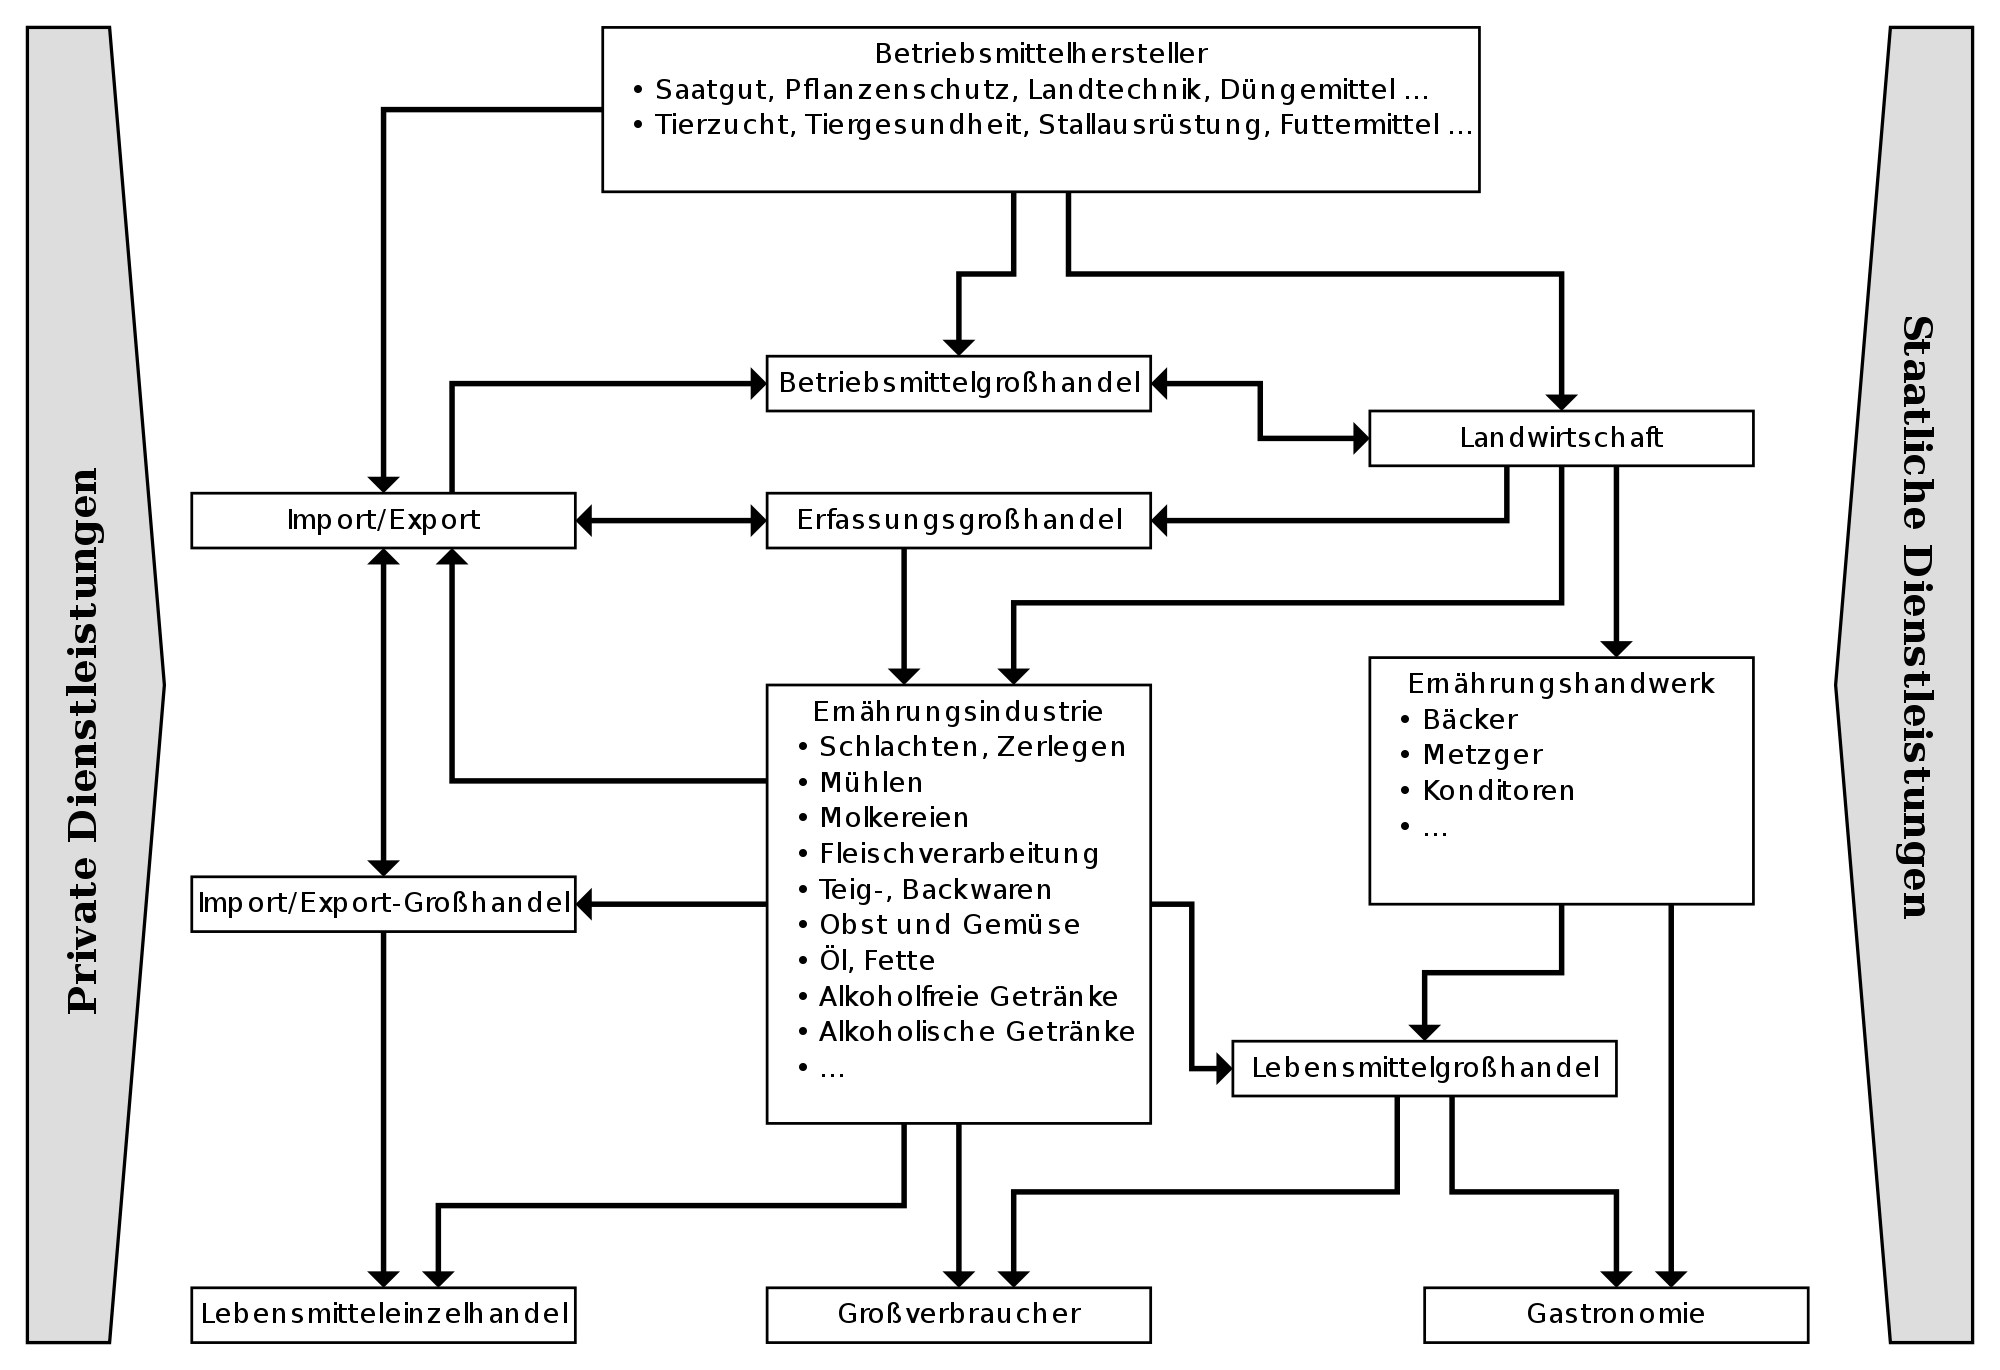
\includegraphics[width=1.0\linewidth]{pictures/system-of-agribusiness}
	\caption[Wertschöpfungskette: Lebensmittelindustrie]{Wertschöpfungskette: Lebensmittelindustrie \textcolor{red}{QUELLE}}
	\label{fig:wkd-Lebensmittelindustrie}
\end{figure}

\paragraph{Downstream Tracing (Abwärts-Rückverfolgbarkeit)}$~~$\\
Als Downstream Tracing wird die Rückverfolgbarkeit ausgehend vom Erzeuger zum Endprodukt bezeichnet. Gegenstand der Rückverfolgung ist typischerweise ein \textit{Los} (\textit{Charge}) oder eine einzelne Einheit eines Produkts. Abhängig vom Grad der Integration innerhalb der Lieferkette lässt sich die Rückverfolgung bis zum Einzelhandel bzw. auch bis zum Endverbraucher durchführen. Zum Einsatz kommt das Downstream Tracing wenn Probleme in Waren zu einem späten Zeitpunkt festgestellt wurden und geprüft werden muss in welchen Endproduktchargen sich hierdurch weitere Probleme ergeben könnten \citep{Trienekens2001, Zailani2010}. \citet{Wegner-Hambloch2004} beschreibt Downstream Tracing als \glqq Ortsbestimmung von bereits hergestellten Produkten zwecks nachträglichen Rückrufs von gesundheitsgefährdenden Produkten\grqq{}.

\paragraph{Upstream Tracing (Aufwärts-Rückverfolgbarkeit)}$~~$\\
Unter Upstream Tracing versteht man die Rückverfolgbarkeit vom Endverbraucher in Richtung des Erzeugers. Tritt ein Problem bei Lebensmittelprodukten auf wird das Upstream Tracing zur Ursachenforschung eingesetzt. So lassen sich Probleme die beispielsweise vom Konsumenten beim Endprodukt oder bei einer Qualitätskontrolle von Teilprodukten festgestellt wurden zurückverfolgen bis zum Urerzeuger \citep{Trienekens2001, Zailani2010}. Nach \citet{Wegner-Hambloch2004} ist Upstream Tracing \glqq die Bestimmung der Produktgeschichte vom Endprodukt [...] bis zu den Futtermitteln.\grqq{}

\subsubsection{Zentrale vs. dezentrale Ansätze}
\textcolor{red}{Unterschied zwischen zentraler Informationssysteme (F-Trace) und dezentraler logischer Systeme (Zugriff auf F-Trace). Letzteres sind nur dem Anschein nach dezentral. Ihre zugrunde liegende Infrastruktur der Informationssysteme ist zentral und wird von einem Intermediär verwaltet und betrieben. Angriffspunkte für Manipulation und Kontrolle eines einzelnen rausarbeiten. \citep{Steins2015, allgemeinefleischerzeitung2011}
Lorem ipsum dolor sit amet, consetetur sadipscing elitr, sed diam nonumy eirmod tempor invidunt ut labore et dolore magna aliquyam erat, sed diam voluptua. At vero eos et accusam et justo duo dolores et ea rebum. Stet clita kasd gubergren, no sea takimata sanctus est Lorem ipsum dolor sit amet. Lorem ipsum dolor sit amet, consetetur sadipscing elitr, sed diam nonumy eirmod tempor invidunt ut labore et dolore magna aliquyam erat, sed diam voluptua. At vero eos et accusam et justo duo dolores et ea rebum. Stet clita kasd gubergren, no sea takimata sanctus est Lorem ipsum dolor sit amet.Lorem ipsum dolor sit amet, consetetur sadipscing elitr, sed diam nonumy eirmod tempor invidunt ut labore et dolore magna aliquyam erat, sed diam voluptua. At vero eos et accusam et justo duo dolores et ea rebum. Stet clita kasd gubergren, no sea takimata sanctus est Lorem ipsum dolor sit amet. Lorem ipsum dolor sit amet, consetetur sadipscing elitr, sed diam nonumy eirmod tempor invidunt ut labore et dolore magna aliquyam erat, sed diam voluptua.}

\subsubsection{Dokumentationspflichten}
Für landwirtschaftliche Waren und daraus hergestellte Nahrungsmittel existieren eine Vielzahl von gesetzlichen Regelungen aus denen Bedingungen und Anforderungen zum Thema Rückverfolgbarkeit abgeleitet werden können. Die VO (EG) Nr. 178/02 \citep{EPER2002} wird in diesem Kontext als Basisverordnung gesehen. Darüber hinaus sind die horizontale Lebensmittelhygieneverordnung sowie die vertikalen Hygieneverordnungen für Fleisch und Fleischerzeugnise, Milch- und Milcherzeugnisse, Fisch und Fischerzeugnisse mit der Vorgabe zur Umsetzung betrieblicher Eigenkontrollen oder Einrichtung eines \acs{haccp}-Systems\footnote{Englisch für \textit{\acf{haccp}}. Beschreibt ein Qualitätskontrollsystem für den sicheren Umgang mit Lebensmitteln durch strukturierte und präventive Maßnahmen zur Verhinderung von Erkrankungen und Verletzungen des Konsumenten.\citep{EPER2004}} elementare Bestandteile eines wirkungsvollen, innerbetrieblichen Rückverfolgungssystems in Lebensmittelbetrieben. Eine verbindliche fünfjährige Speicherung von Daten der Transaktionen bezüglich der Lieferanten und Abnehmer ist ebenfalls festgelegt.\\

\noindent
Weitere Regelungen zur Rückverfolgbarkeit für die EU:
\begin{itemize}
  \item Rindfleischetikettierungs-VO (EWG) Nr. 1760/2000
  \item EU-Öko-VO (EWG) 2092/91
  \item EU-Verordnung über amtliche Futter- und Lebensmittelkontrollen (Vorschlag vom 5. Februar 2003)
  \item Vermarktungsnormen für Eier 1907/90/EWG
\end{itemize}
Nationale Regelungen für Deutschland:
\begin{itemize}
  \item \acf{lmkv}
  \item \acf{lkv}
  \item verschiedene Fleisch- und Geflügelfleisch-Hygienevorschriften
  \item Weingesetz und Weinwirtschaftsgesetz
  \item Handelsklassenrecht
  \item \acf{lmbg}
\end{itemize}
Über die gesetzlichen Regelungen hinaus gelten verbindliche Standards der Handelsseite, die übergreifend von der \ac{gfsi} vorgegeben werden. Der in Deutschland meist gefragte \ac{ifs}, der Standard des \ac{brc} für Lieferanten nach England und diverse andere Standards definieren das detaillierte Anforderungsniveau transparenter Warenströme aus Handelssicht für den Hersteller.

\subsubsection{???Besonderheiten der Fleischwarenindustrie???}
\textcolor{red}{Lorem ipsum dolor sit amet, consetetur sadipscing elitr, sed diam nonumy eirmod tempor invidunt ut labore et dolore magna aliquyam erat, sed diam voluptua. At vero eos et accusam et justo duo dolores et ea rebum. Stet clita kasd gubergren, no sea takimata sanctus est Lorem ipsum dolor sit amet. Lorem ipsum dolor sit amet, consetetur sadipscing elitr, sed diam nonumy eirmod tempor invidunt ut labore et dolore magna aliquyam erat, sed diam voluptua. At vero eos et accusam et justo duo dolores et ea rebum. Stet clita kasd gubergren, no sea takimata sanctus est Lorem ipsum dolor sit amet.Lorem ipsum dolor sit amet, consetetur sadipscing elitr, sed diam nonumy eirmod tempor invidunt ut labore et dolore magna aliquyam erat, sed diam voluptua. At vero eos et accusam et justo duo dolores et ea rebum. Stet clita kasd gubergren, no sea takimata sanctus est Lorem ipsum dolor sit amet. Lorem ipsum dolor sit amet, consetetur sadipscing elitr, sed diam nonumy eirmod tempor invidunt ut labore et dolore magna aliquyam erat, sed diam voluptua. At vero eos et accusam et justo duo dolores et ea rebum. Stet clita kasd gubergren, no sea takimata sanctus est Lorem ipsum dolor sit amet. Lorem ipsum dolor sit amet, consetetur sadipscing elitr, sed diam nonumy eirmod tempor invidunt ut labore et dolore magna aliquyam erat, sed diam voluptua. At vero eos et accusam et justo duo dolores et ea rebum. Stet clita kasd gubergren, no sea takimata sanctus est Lorem ipsum dolor sit amet.}
